\documentclass[a4paper, 10pt]{article}

\usepackage[utf8x]{inputenc}
\usepackage[english, russian, ukrainian]{babel}
\usepackage{cmap}
\usepackage{mathtext}
\usepackage[T2A]{fontenc}

\usepackage{graphicx}
\usepackage{float}
\usepackage{bytefield}
\usepackage{multicol}
\usepackage{multirow}

\usepackage{geometry}
\geometry{top = 2cm}
\geometry{bottom = 2cm}
\geometry{left = 3cm}
\geometry{right = 1.5cm}

\begin{document}
\begin{titlepage}
\begin{center}
\large{
Міністерство освіти і науки, молоді та спорту України\\
Національний технічний університет України\\
``Київський політехнічний інститут''\\
Факультет прикладної математики\\
Кафедра спеціалізованих комп’ютерних систем\\
}

\vfill

\large{\bf{
Лабораторна робота №2\\
Дисципліна:\\
``Архітектура комп'ютерів''\\
Тема:\\
``Блоки мікропрограмного управління''\\
}}

\vfill

\begin{table}[h]
\centering
\begin{tabular}{lp{4cm}l}
Виконав:&&Перевірив:\\
Студент групи КВ--92&&Жабін В. І.\\
Гуль О. В.&&\\
Залікова книжка № КВ--9203&&\\
\end{tabular}
\end{table}

\vfill

Київ \the\year
\end{center}
\end{titlepage}
\newpage

\section{Мета}
Дослідити засоби побудови блоків мікропрограмного управління. Одержати навички в проектуванні й налагодженні схем пристроїв управління з мікропрограмним управлінням.

\section{Завдання}
\begin{enumerate}
    \item Варіанти завдання визначаються молодшими розрядами $a_{7},\cdots,a_{1}$ двійкового номера залікової книжки.
    \item Розробити структурну схему операційного пристрою та змістовний мікроалгоритм обробки додатних чисел відповідно до завдання наведеного у табл. 3.14. Для побудови схеми використати комбінаційний суматор, регістр--лічильник циклів та асинхронні регістри, що мають входи управління зсувами і занесенням інформації. На структурный схемі повинні бути зазначені розрядність регістрів та шин.
    \item Розробити функціональну схему операційного пристрою.
    \item Виконати логічне моделювання роботи операційного пристрою за допомогою цифрової діаграми для вибраних значень операндів і їх розрядності.
	\item Побудувати структурну і функціональну схему БМУ, а також карту програмування ПМК для мікроалгоритму виконання заданої операції.
	\item Використувати горизонтальне програмування зони управляючих сигналів. Врахувати дані, наведені у табл. 3.15–-3.16.
\end{enumerate}

\noindent
Варіант: $9203=10001111110011_2$.\\
$a_{7},\cdots,a_{1}=1110011.$\\
Функція: 3--й спосіб множення.\\
Розрядність операндів (без знаку): 7.\\
Спосіб адресації мікрокоманд: примусовий.\\
Структура ПМК: лінійна.\\
Ємність ПМК, слова: 32.\\
Використати зону $\beta4$ для перевірки слова МК: на парність.\\
Тривалість мікрооперації підсумовування, такти: 5.\\
Інщі мікрооперації виконуються за один такт.\\
Врахувати, що мікрооперації на регістрах виконуються за перепадом управляючих сигналів з 1 в 0.

\section{Короткі теоретичні відомості}
БМУ функціонує у відповідності з принципом мікропрограмного управління. МК розміщуються у пам’яті мікрокоманд. Поля МК є сигналами управління пристроями, також
вони визначають тривалість цих сигналів та адресу наступної МК. Такі сигнали формуюит з використанням логічнх умов, що надходять на вхід схеми.

\section{Порядок виконання роботи}
\begin{enumerate}
    \item Використовуючи моделюючу систему AFDK (ПРОГМОЛС 2.0) побудувати і налагодити пристрій для виконання заданої операції. Опис програмного комплексу ПРОГМОЛС 2.0 наведений у додатку.
    \item На спроектованому пристрої виконати числовий приклад і порівняти результат з одержаним при логічному моделюванні.
\end{enumerate}

\section{Виконання завдання}
$Z=Y\cdot X.$\\
RG3~-- регістр множеного.\\
RG2~-- регістр множника. МО зсуву вліво.\\
RG1~-- регістр добутку. МО зсуву вліво.\\
SM~-- комбінаційний суматор.\\
CT~-- регістр--лічильник тактів. Лічильник, формує ознаку $CT=n$.\\

\begin{figure}[h!]
\begin{center}
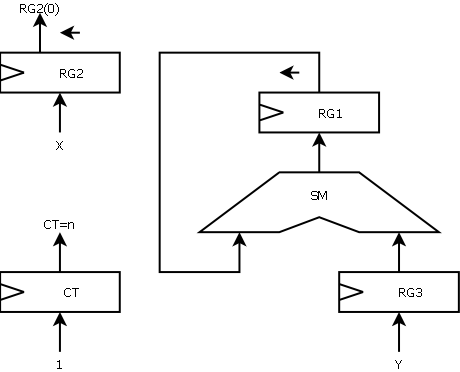
\includegraphics[scale=0.5]{od.png}
\caption{Схема операційного пристрою.}
\end{center}
\end{figure}

\begin{figure}[H]
\begin{center}
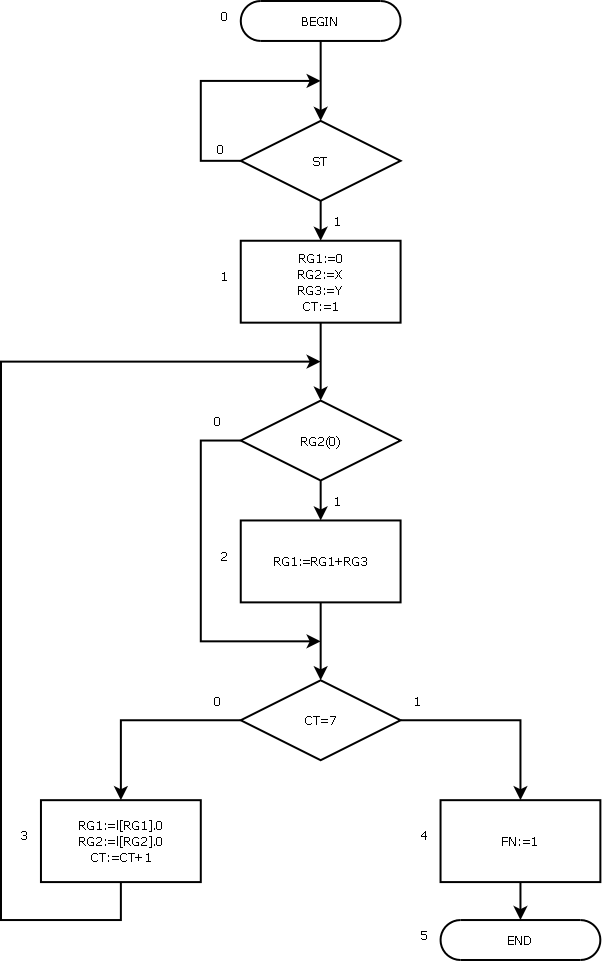
\includegraphics[scale=0.25]{f_alg.png}
\caption{Функціональний мікроалгоритм.}
\end{center}
\end{figure}

\begin{figure}[H]
\begin{center}
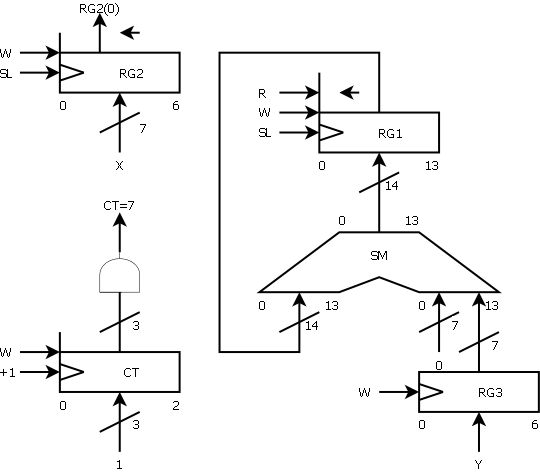
\includegraphics[scale=0.5]{fs.png}
\caption{Функціональна схема операційного пристрою.}
\end{center}
\end{figure}

\begin{figure}[H]
\begin{center}
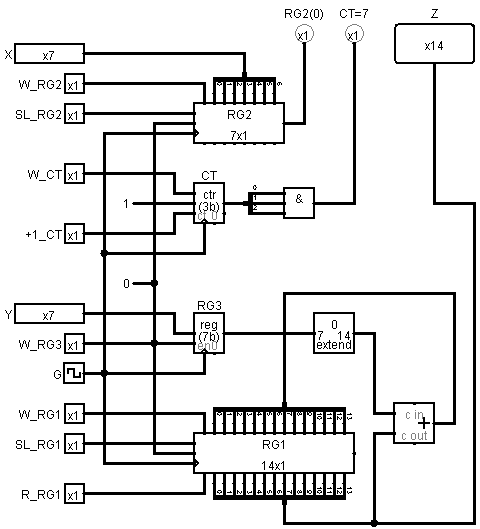
\includegraphics[scale=0.75, angle=0]{od_circ.png}
\caption{Зiбрана функціональна схема операційного пристрою.}
\end{center}
\end{figure}

\noindent
$Z=Y\cdot X.$\\
$Y=10=0001010_{2}$\\
$X=11=0001011_{2}$\\
\begin{table}[h!]
\centering
\begin{tabular}{|cc|c|c|c|c|}
\hline
RG2(0) & RG2 & RG3 & RG1 & CT & №MO\\
\hline
0&001011&0001010&00000000000000&001&1\\
0&010110&0001010&00000000000000&010&3\\
0&101100&0001010&00000000000000&011&3\\
1&011000&0001010&00000000000000&100&3\\
1&011000&0001010&00000000001010&100&2\\
0&110000&0001010&00000000010100&101&3\\
1&100000&0001010&00000000101000&110&3\\
1&100000&0001010&00000000110010&110&2\\
1&000000&0001010&00000001100100&111&3\\
1&000000&0001010&00000001101110&111&2\\
\hline
\end{tabular}
\caption{Дiаграма станiв регiстрiв при виконаннi алгоритму.}
\end{table}

\begin{table}[h!]
\centering
\begin{tabular}{|c|c|c|}
\hline
Елемент & Мікрооперація & Управляючий сигнал\\
\hline
RG1 & Скидання   & R    $1\to0$ \\
RG1 & Запис      & W    $1\to0$ \\
RG1 & Зсув вліво & SL   $1\to0$ \\
\hline
RG2 & Запис      & W    $1\to0$ \\
RG2 & Зсув вліво & SL   $1\to0$ \\
\hline
RG3 & Запис      & W    $1\to0$ \\
\hline
CT  & Запис      & W    $1\to0$ \\
CT  & Інкремент  & $+1$ $1\to0$ \\
\hline
\end{tabular}
\caption{Перелік управляючих сигналів елементів.}
\end{table}

\begin{figure}[H]
\begin{center}
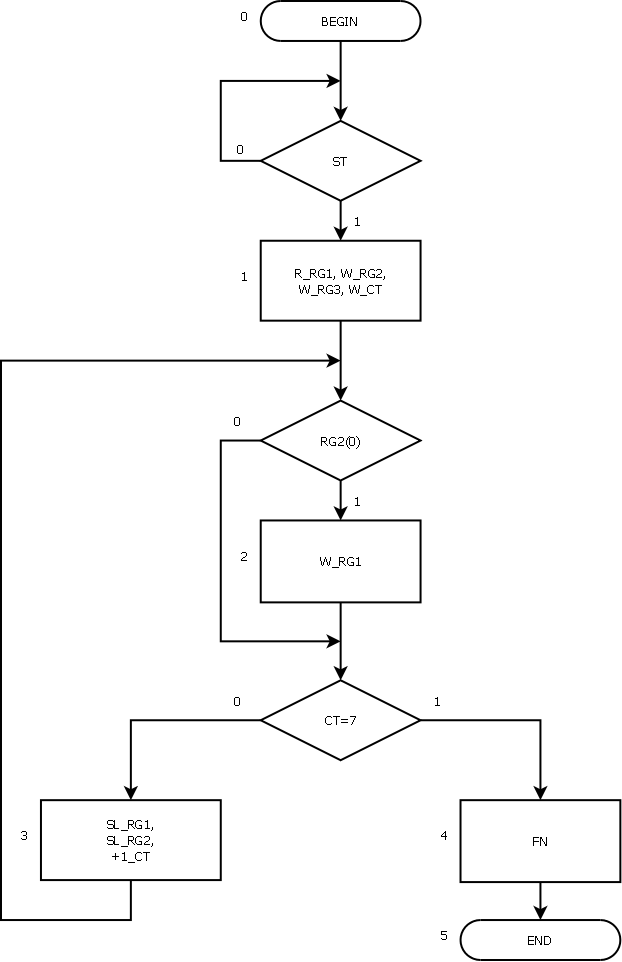
\includegraphics[scale=0.25]{fs_alg.png}
\caption{Функціонально--структурний мікроалгоритм.}
\end{center}
\end{figure}

\begin{table}[h!]
\centering
\begin{tabular}{|c|c|c|}
\hline
№МО & Мікрооперації & код\\
\hline
1 & $R_{RG1}, W_{RG2}, W_{RG3}, W_{CT}$ & $Y_1$ \\
2 & $W_{RG1}$                           & $Y_2$\\
3 & $SL_{RG1}, SL_{RG2}, +1_{CT}$       & $Y_3$ \\
4 & $FN$                                & $Y_4$ \\
\hline
\end{tabular}
\caption{Кодування сигналів управління.}
\end{table}

\begin{table}[h!]
\centering
\begin{tabular}{|c|c|}
\hline
Умова & Код\\
\hline
Пуск & ST \\
\hline
Кінець & FN\\
\hline
Лічильник циклів дорахував до n & CT=n\\
\hline
Старший розряд RG2. & RG2(0)\\
\hline
\end{tabular}
\caption{Кодування логічних умов.}
\end{table}

\begin{figure}[H]
\begin{center}
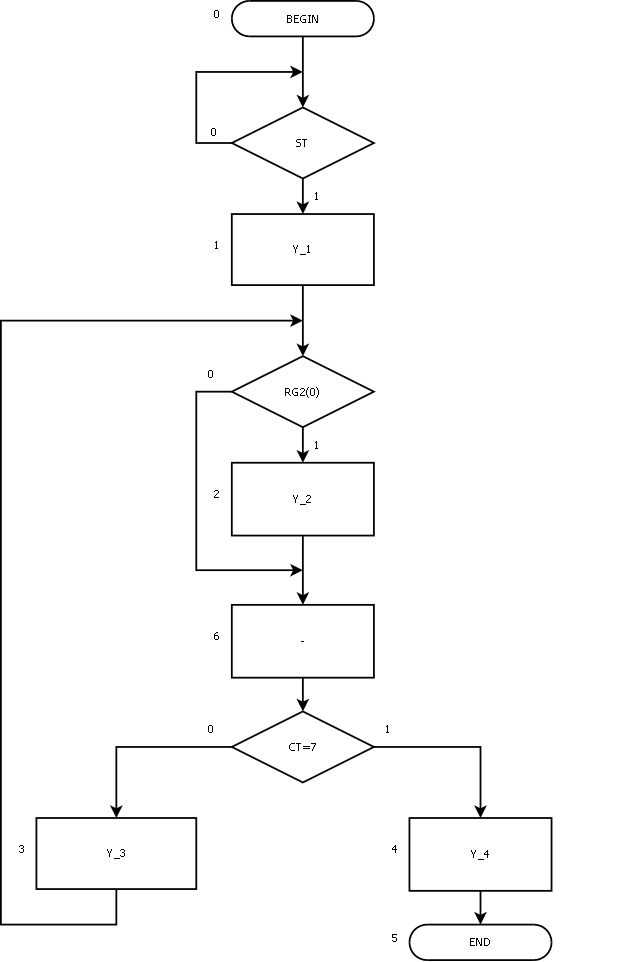
\includegraphics[scale=0.25]{fsz_alg.png}
\caption{Закодований функціонально--структурний мікроалгоритм.}
\end{center}
\end{figure}

\begin{figure}[H]
\begin{center}
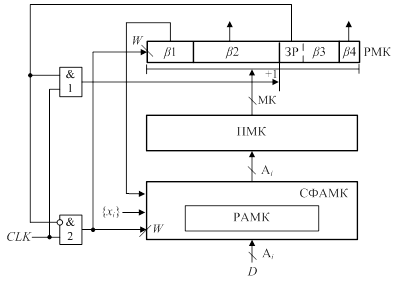
\includegraphics[scale=1.0]{mpcu1.png}
\caption{Структурна схема БМУ з урахуванням зони затримки УС.}
\end{center}
\end{figure}

\begin{figure}[H]
\begin{center}
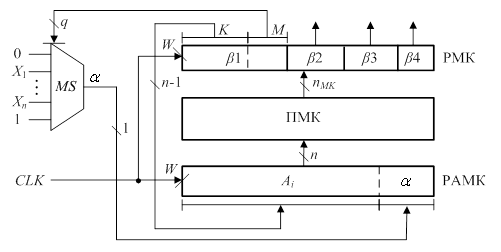
\includegraphics[scale=1.0]{mpcu2.png}
\caption{Структурна схема БМУ з примусовою адресацією.}
\end{center}
\end{figure}

Формат зони $\beta1$:\\
$\textnormal{Розрядність адрес ПМК}       : n_a        = \lceil log_{2}32 \rceil = 5 ;$\\
$\textnormal{Ширина поля K зони $\beta1$} : n_K        = n_a - 1 = 5 - 1 = 4         ;$\\
$\textnormal{Кількість логічних умов}     : n_l        = 2 + 3 = 5                   ;$\\
$\textnormal{Ширина поля M зони $\beta1$} : n_M        = \lceil log_{2}5 \rceil = 3  ;$\\
$\textnormal{Ширина поля зони $\beta1$}   : n_{\beta1} = n_K + n_M = 4 + 3 = 7       ;$\\

\begin{table}[h!]
\centering
\begin{tabular}{|c|c|}
\hline
$m_2 m_1 m_0$ & Умова\\
\hline
000 & 0  \\
001 & ST \\
010 & RG2(0) \\
011 & CT=n \\
111 & 1 \\
\hline
\end{tabular}
\caption{Кодування поля M.}
\end{table}

Формат зони $\beta2$:\\
$n_{\beta2} = 4;$\\

Формат зони $\beta3$:\\
$\Delta t_{max} = 5;$\\
$n_{\beta3} = \lceil log_{2}(5) \rceil + 1 = 4 ;$\\

Формат зони $\beta4$:\\
$n_{\beta4} = 1 ;$\\

Формат мiкрокоманди ($n_{МК} = 16$):
\\
\\
\begin{bytefield}[endianness=big, bitwidth=14pt]{16}
	\bitheader{0-15} \\
	\bitbox{7}{$\beta1$} & \bitbox{4}{$\beta2$} & \bitbox{4}{$\beta3$} & \bitbox{1}{$\beta4$} \\
	\bitbox{3}{M} & \bitbox{4}{K} & \bitbox{1}{$Y_1$} & \bitbox{1}{$Y_2$} & \bitbox{1}{$Y_3$} & \bitbox{1}{$Y_4$} & \bitbox{1}{ЗР} & \bitbox{3}{} & \bitbox{1}{} \\
	\bitheader{0-15}
\end{bytefield}

Переходи між командами:\\
$0 \to 0, 0 \to 1$\\
$1 \to 2, 1 \to 6$\\
$2 \to 6$\\
$6 \to 4, 6 \to 3$\\
$3 \to 2, 3 \to 6$\\
$4 \to 5$\\
$5 \to 5$\\

Вимоги щодо розміщення МК в ПМК:\\
$0 | 1;$ \\
$6 | 2;$ \\
$3 | 4;$ \\

\begin{table}[H]
\centering
\begin{tabular}{|c|c|}
\hline
Адреса & ПМК \\
\hline
00000 & П(0) \\
00001 & 1 \\
00010 & 6 \\
00011 & 2 \\
00100 & 3 \\
00101 & 4 \\
00110 & К(5) \\
\hline
\end{tabular}
\caption{Розмішення команд в ПМК.}
\end{table}

\begin{table}[H]
\centering
\begin{tabular}{|c|c|c|c|c|c|c|c|}
\hline
\multirow{2}{*}{№ МК} &
\multirow{2}{*}{Адреса} &
\multicolumn{2}{|c|}{$\beta1$} &
$\beta2$ & 
\multicolumn{2}{|c|}{$\beta3$} &
\multirow{2}{*}{$\beta4$} \\
\cline{3-7}
      &      &  K   &  M  & $Y_1 Y_2 Y_3 Y_4$ & ЗР &     & \\
\hline
00000 & П(0) & 0000 & 001 & 0000           & 1  & 111 & 1 \\
00001 & 1    & 0001 & 010 & 1000           & 1  & 111 & 1 \\
00010 & 6    & 0010 & 011 & 0000           & 1  & 111 & 1 \\
00011 & 2    & 0001 & 000 & 0100           & 1  & 100 & 0 \\
00100 & 3    & 0001 & 010 & 0010           & 1  & 111 & 0 \\
00101 & 4    & 0011 & 000 & 0001           & 1  & 111 & 1 \\
00110 & К(5) & 0011 & 000 & 0001           & 1  & 111 & 1 \\
\hline
\end{tabular}
\caption{Карта програмування БМУ.}
\end{table}

\begin{figure}[H]
\begin{center}
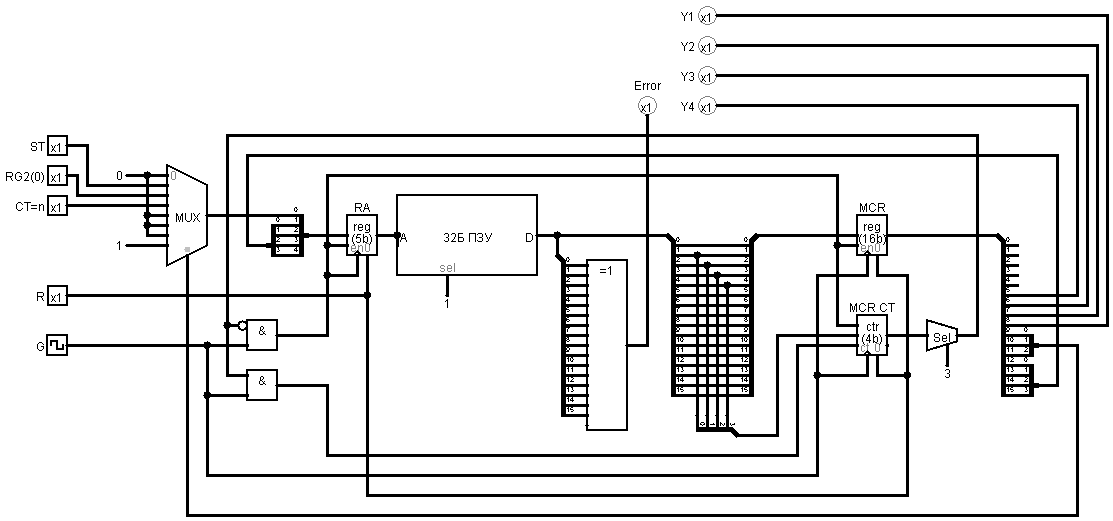
\includegraphics[scale=0.6, angle=90]{mpcu_circ.png}
\caption{Зiбраний БМУ.}
\end{center}
\end{figure}

\begin{figure}[H]
\begin{center}
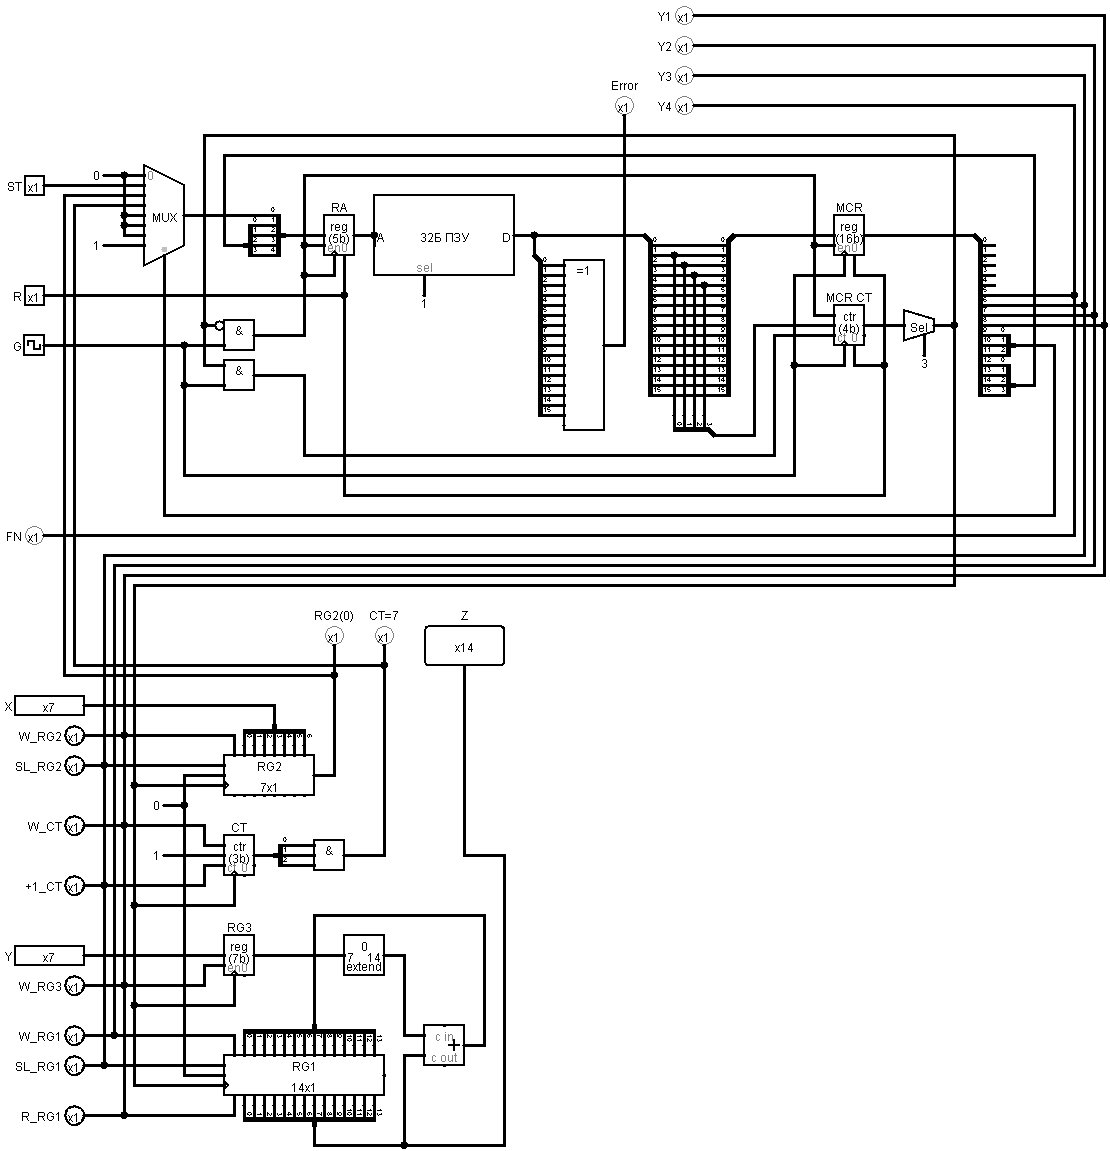
\includegraphics[scale=0.4, angle=90]{lab2.png}
\caption{Зiбрана схема.}
\end{center}
\end{figure}


\begin{table}[h!]
\tiny
\centering
\setlength{\tabcolsep}{1pt}
\begin{tabular}{|c|c|c|c|c|c|c|c|c|c|c|c|c|c|c|c|c|c|c|c|c|}
\hline
ST& R & G & CT& RG1            & RG2     & RG3&$RG2(0)$&$CT=7$&$R_{RG1}$&$W_{RG1}$&$SL_{RG1}$&$W_{RG2}$&$SL_{RG2}$&$W_{CT}$ &$+1_{CT}$ &$W_{RG3}$ &FN \\ \hline
0 & 0 & 0 & 111&00000000000000 & 0000000 & 0000000 &  0 & 1 & 0 & 0 & 0 & 0 & 0 & 0 & 0 & 0 &  0\\ \hline
0 & 1 & 0 & 111&00000000000000 & 0000000 & 0000000 &  0 & 1 & 0 & 0 & 0 & 0 & 0 & 0 & 0 & 0 &  0\\ \hline
0 & 0 & 0 & 111&00000000000000 & 0000000 & 0000000 &  0 & 1 & 0 & 0 & 0 & 0 & 0 & 0 & 0 & 0 &  0\\ \hline
0 & 1 & 0 & 111&00000000000000 & 0000000 & 0000000 &  0 & 1 & 0 & 0 & 0 & 0 & 0 & 0 & 0 & 0 &  0\\ \hline
0 & 0 & 0 & 111&00000000000000 & 0000000 & 0000000 &  0 & 1 & 0 & 0 & 0 & 0 & 0 & 0 & 0 & 0 &  0\\ \hline
0 & 0 & 1 & 111&00000000000000 & 0000000 & 0000000 &  0 & 1 & 0 & 0 & 0 & 0 & 0 & 0 & 0 & 0 &  0\\ \hline
0 & 0 & 0 & 111&00000000000000 & 0000000 & 0000000 &  0 & 1 & 0 & 0 & 0 & 0 & 0 & 0 & 0 & 0 &  0\\ \hline
0 & 0 & 1 & 111&00000000000000 & 0000000 & 0000000 &  0 & 1 & 0 & 0 & 0 & 0 & 0 & 0 & 0 & 0 &  0\\ \hline
0 & 0 & 0 & 111&00000000000000 & 0000000 & 0000000 &  0 & 1 & 0 & 0 & 0 & 0 & 0 & 0 & 0 & 0 &  0\\ \hline
1 & 0 & 0 & 111&00000000000000 & 0000000 & 0000000 &  0 & 1 & 0 & 0 & 0 & 0 & 0 & 0 & 0 & 0 &  0\\ \hline
1 & 0 & 1 & 111&00000000000000 & 0000000 & 0000000 &  0 & 1 & 0 & 0 & 0 & 0 & 0 & 0 & 0 & 0 &  0\\ \hline
1 & 0 & 0 & 111&00000000000000 & 0000000 & 0000000 &  0 & 1 & 1 & 0 & 0 & 1 & 0 & 1 & 0 & 1 &  0\\ \hline
1 & 0 & 1 & 111&00000000000000 & 0000000 & 0000000 &  0 & 1 & 1 & 0 & 0 & 1 & 0 & 1 & 0 & 1 &  0\\ \hline
1 & 0 & 0 & 001&00000000000000 & 0000011 & 0000100 &  0 & 0 & 1 & 0 & 0 & 1 & 0 & 1 & 0 & 1 &  0\\ \hline
0 & 0 & 0 & 001&00000000000000 & 0000011 & 0000100 &  0 & 0 & 1 & 0 & 0 & 1 & 0 & 1 & 0 & 1 &  0\\ \hline
0 & 0 & 1 & 001&00000000000000 & 0000011 & 0000100 &  0 & 0 & 1 & 0 & 0 & 1 & 0 & 1 & 0 & 1 &  0\\ \hline
0 & 0 & 0 & 001&00000000000000 & 0000011 & 0000100 &  0 & 0 & 0 & 0 & 0 & 0 & 0 & 0 & 0 & 0 &  0\\ \hline
0 & 0 & 1 & 001&00000000000000 & 0000011 & 0000100 &  0 & 0 & 0 & 0 & 0 & 0 & 0 & 0 & 0 & 0 &  0\\ \hline
0 & 0 & 0 & 001&00000000000000 & 0000011 & 0000100 &  0 & 0 & 0 & 0 & 0 & 0 & 0 & 0 & 0 & 0 &  0\\ \hline
0 & 0 & 1 & 001&00000000000000 & 0000011 & 0000100 &  0 & 0 & 0 & 0 & 0 & 0 & 0 & 0 & 0 & 0 &  0\\ \hline
0 & 0 & 0 & 001&00000000000000 & 0000011 & 0000100 &  0 & 0 & 0 & 0 & 1 & 0 & 1 & 0 & 1 & 0 &  0\\ \hline
0 & 0 & 1 & 001&00000000000000 & 0000011 & 0000100 &  0 & 0 & 0 & 0 & 1 & 0 & 1 & 0 & 1 & 0 &  0\\ \hline
0 & 0 & 0 & 010&00000000000000 & 0000110 & 0000100 &  0 & 0 & 0 & 0 & 1 & 0 & 1 & 0 & 1 & 0 &  0\\ \hline
0 & 0 & 1 & 010&00000000000000 & 0000110 & 0000100 &  0 & 0 & 0 & 0 & 1 & 0 & 1 & 0 & 1 & 0 &  0\\ \hline
0 & 0 & 0 & 010&00000000000000 & 0000110 & 0000100 &  0 & 0 & 0 & 0 & 0 & 0 & 0 & 0 & 0 & 0 &  0\\ \hline
0 & 0 & 1 & 010&00000000000000 & 0000110 & 0000100 &  0 & 0 & 0 & 0 & 0 & 0 & 0 & 0 & 0 & 0 &  0\\ \hline
0 & 0 & 0 & 010&00000000000000 & 0000110 & 0000100 &  0 & 0 & 0 & 0 & 0 & 0 & 0 & 0 & 0 & 0 &  0\\ \hline
0 & 0 & 1 & 010&00000000000000 & 0000110 & 0000100 &  0 & 0 & 0 & 0 & 0 & 0 & 0 & 0 & 0 & 0 &  0\\ \hline
0 & 0 & 0 & 010&00000000000000 & 0000110 & 0000100 &  0 & 0 & 0 & 0 & 1 & 0 & 1 & 0 & 1 & 0 &  0\\ \hline
0 & 0 & 1 & 010&00000000000000 & 0000110 & 0000100 &  0 & 0 & 0 & 0 & 1 & 0 & 1 & 0 & 1 & 0 &  0\\ \hline
0 & 0 & 0 & 011&00000000000000 & 0001100 & 0000100 &  0 & 0 & 0 & 0 & 1 & 0 & 1 & 0 & 1 & 0 &  0\\ \hline
0 & 0 & 1 & 011&00000000000000 & 0001100 & 0000100 &  0 & 0 & 0 & 0 & 1 & 0 & 1 & 0 & 1 & 0 &  0\\ \hline
0 & 0 & 0 & 011&00000000000000 & 0001100 & 0000100 &  0 & 0 & 0 & 0 & 0 & 0 & 0 & 0 & 0 & 0 &  0\\ \hline
0 & 0 & 1 & 011&00000000000000 & 0001100 & 0000100 &  0 & 0 & 0 & 0 & 0 & 0 & 0 & 0 & 0 & 0 &  0\\ \hline
0 & 0 & 0 & 011&00000000000000 & 0001100 & 0000100 &  0 & 0 & 0 & 0 & 0 & 0 & 0 & 0 & 0 & 0 &  0\\ \hline
0 & 0 & 1 & 011&00000000000000 & 0001100 & 0000100 &  0 & 0 & 0 & 0 & 0 & 0 & 0 & 0 & 0 & 0 &  0\\ \hline
0 & 0 & 0 & 011&00000000000000 & 0001100 & 0000100 &  0 & 0 & 0 & 0 & 1 & 0 & 1 & 0 & 1 & 0 &  0\\ \hline
0 & 0 & 1 & 011&00000000000000 & 0001100 & 0000100 &  0 & 0 & 0 & 0 & 1 & 0 & 1 & 0 & 1 & 0 &  0\\ \hline
0 & 0 & 0 & 100&00000000000000 & 0011000 & 0000100 &  0 & 0 & 0 & 0 & 1 & 0 & 1 & 0 & 1 & 0 &  0\\ \hline
0 & 0 & 1 & 100&00000000000000 & 0011000 & 0000100 &  0 & 0 & 0 & 0 & 1 & 0 & 1 & 0 & 1 & 0 &  0\\ \hline
0 & 0 & 0 & 100&00000000000000 & 0011000 & 0000100 &  0 & 0 & 0 & 0 & 0 & 0 & 0 & 0 & 0 & 0 &  0\\ \hline
0 & 0 & 1 & 100&00000000000000 & 0011000 & 0000100 &  0 & 0 & 0 & 0 & 0 & 0 & 0 & 0 & 0 & 0 &  0\\ \hline
0 & 0 & 0 & 100&00000000000000 & 0011000 & 0000100 &  0 & 0 & 0 & 0 & 0 & 0 & 0 & 0 & 0 & 0 &  0\\ \hline
0 & 0 & 1 & 100&00000000000000 & 0011000 & 0000100 &  0 & 0 & 0 & 0 & 0 & 0 & 0 & 0 & 0 & 0 &  0\\ \hline
0 & 0 & 0 & 100&00000000000000 & 0011000 & 0000100 &  0 & 0 & 0 & 0 & 1 & 0 & 1 & 0 & 1 & 0 &  0\\ \hline
0 & 0 & 1 & 100&00000000000000 & 0011000 & 0000100 &  0 & 0 & 0 & 0 & 1 & 0 & 1 & 0 & 1 & 0 &  0\\ \hline
0 & 0 & 0 & 101&00000000000000 & 0110000 & 0000100 &  0 & 0 & 0 & 0 & 1 & 0 & 1 & 0 & 1 & 0 &  0\\ \hline
0 & 0 & 1 & 101&00000000000000 & 0110000 & 0000100 &  0 & 0 & 0 & 0 & 1 & 0 & 1 & 0 & 1 & 0 &  0\\ \hline
0 & 0 & 0 & 101&00000000000000 & 0110000 & 0000100 &  0 & 0 & 0 & 0 & 0 & 0 & 0 & 0 & 0 & 0 &  0\\ \hline
0 & 0 & 1 & 101&00000000000000 & 0110000 & 0000100 &  0 & 0 & 0 & 0 & 0 & 0 & 0 & 0 & 0 & 0 &  0\\ \hline
0 & 0 & 0 & 101&00000000000000 & 0110000 & 0000100 &  0 & 0 & 0 & 0 & 0 & 0 & 0 & 0 & 0 & 0 &  0\\ \hline
0 & 0 & 1 & 101&00000000000000 & 0110000 & 0000100 &  0 & 0 & 0 & 0 & 0 & 0 & 0 & 0 & 0 & 0 &  0\\ \hline
0 & 0 & 0 & 101&00000000000000 & 0110000 & 0000100 &  0 & 0 & 0 & 0 & 1 & 0 & 1 & 0 & 1 & 0 &  0\\ \hline
0 & 0 & 1 & 101&00000000000000 & 0110000 & 0000100 &  0 & 0 & 0 & 0 & 1 & 0 & 1 & 0 & 1 & 0 &  0\\ \hline
0 & 0 & 0 & 110&00000000000000 & 1100000 & 0000100 &  1 & 0 & 0 & 0 & 1 & 0 & 1 & 0 & 1 & 0 &  0\\ \hline
0 & 0 & 1 & 110&00000000000000 & 1100000 & 0000100 &  1 & 0 & 0 & 0 & 1 & 0 & 1 & 0 & 1 & 0 &  0\\ \hline
0 & 0 & 0 & 110&00000000000000 & 1100000 & 0000100 &  1 & 0 & 0 & 1 & 0 & 0 & 0 & 0 & 0 & 0 &  0\\ \hline
0 & 0 & 1 & 110&00000000000000 & 1100000 & 0000100 &  1 & 0 & 0 & 1 & 0 & 0 & 0 & 0 & 0 & 0 &  0\\ \hline
0 & 0 & 0 & 110&00000000000000 & 1100000 & 0000100 &  1 & 0 & 0 & 1 & 0 & 0 & 0 & 0 & 0 & 0 &  0\\ \hline
0 & 0 & 1 & 110&00000000000000 & 1100000 & 0000100 &  1 & 0 & 0 & 1 & 0 & 0 & 0 & 0 & 0 & 0 &  0\\ \hline
0 & 0 & 0 & 110&00000000000000 & 1100000 & 0000100 &  1 & 0 & 0 & 1 & 0 & 0 & 0 & 0 & 0 & 0 &  0\\ \hline
0 & 0 & 1 & 110&00000000000000 & 1100000 & 0000100 &  1 & 0 & 0 & 1 & 0 & 0 & 0 & 0 & 0 & 0 &  0\\ \hline
0 & 0 & 0 & 110&00000000000000 & 1100000 & 0000100 &  1 & 0 & 0 & 1 & 0 & 0 & 0 & 0 & 0 & 0 &  0\\ \hline
0 & 0 & 1 & 110&00000000000000 & 1100000 & 0000100 &  1 & 0 & 0 & 1 & 0 & 0 & 0 & 0 & 0 & 0 &  0\\ \hline
0 & 0 & 0 & 110&00000000000100 & 1100000 & 0000100 &  1 & 0 & 0 & 1 & 0 & 0 & 0 & 0 & 0 & 0 &  0\\ \hline
0 & 0 & 1 & 110&00000000000100 & 1100000 & 0000100 &  1 & 0 & 0 & 1 & 0 & 0 & 0 & 0 & 0 & 0 &  0\\ \hline
0 & 0 & 0 & 110&00000000000100 & 1100000 & 0000100 &  1 & 0 & 0 & 0 & 0 & 0 & 0 & 0 & 0 & 0 &  0\\ \hline
0 & 0 & 1 & 110&00000000000100 & 1100000 & 0000100 &  1 & 0 & 0 & 0 & 0 & 0 & 0 & 0 & 0 & 0 &  0\\ \hline
0 & 0 & 0 & 110&00000000000100 & 1100000 & 0000100 &  1 & 0 & 0 & 0 & 0 & 0 & 0 & 0 & 0 & 0 &  0\\ \hline
0 & 0 & 1 & 110&00000000000100 & 1100000 & 0000100 &  1 & 0 & 0 & 0 & 0 & 0 & 0 & 0 & 0 & 0 &  0\\ \hline
0 & 0 & 0 & 110&00000000000100 & 1100000 & 0000100 &  1 & 0 & 0 & 0 & 1 & 0 & 1 & 0 & 1 & 0 &  0\\ \hline
0 & 0 & 1 & 110&00000000000100 & 1100000 & 0000100 &  1 & 0 & 0 & 0 & 1 & 0 & 1 & 0 & 1 & 0 &  0\\ \hline
0 & 0 & 0 & 111&00000000001000 & 1000000 & 0000100 &  1 & 1 & 0 & 0 & 1 & 0 & 1 & 0 & 1 & 0 &  0\\ \hline
0 & 0 & 1 & 111&00000000001000 & 1000000 & 0000100 &  1 & 1 & 0 & 0 & 1 & 0 & 1 & 0 & 1 & 0 &  0\\ \hline
0 & 0 & 0 & 111&00000000001000 & 1000000 & 0000100 &  1 & 1 & 0 & 1 & 0 & 0 & 0 & 0 & 0 & 0 &  0\\ \hline
0 & 0 & 1 & 111&00000000001000 & 1000000 & 0000100 &  1 & 1 & 0 & 1 & 0 & 0 & 0 & 0 & 0 & 0 &  0\\ \hline
0 & 0 & 0 & 111&00000000001000 & 1000000 & 0000100 &  1 & 1 & 0 & 1 & 0 & 0 & 0 & 0 & 0 & 0 &  0\\ \hline
0 & 0 & 1 & 111&00000000001000 & 1000000 & 0000100 &  1 & 1 & 0 & 1 & 0 & 0 & 0 & 0 & 0 & 0 &  0\\ \hline
0 & 0 & 0 & 111&00000000001000 & 1000000 & 0000100 &  1 & 1 & 0 & 1 & 0 & 0 & 0 & 0 & 0 & 0 &  0\\ \hline
0 & 0 & 1 & 111&00000000001000 & 1000000 & 0000100 &  1 & 1 & 0 & 1 & 0 & 0 & 0 & 0 & 0 & 0 &  0\\ \hline
0 & 0 & 0 & 111&00000000001000 & 1000000 & 0000100 &  1 & 1 & 0 & 1 & 0 & 0 & 0 & 0 & 0 & 0 &  0\\ \hline
0 & 0 & 1 & 111&00000000001000 & 1000000 & 0000100 &  1 & 1 & 0 & 1 & 0 & 0 & 0 & 0 & 0 & 0 &  0\\ \hline
0 & 0 & 0 & 111&00000000001100 & 1000000 & 0000100 &  1 & 1 & 0 & 1 & 0 & 0 & 0 & 0 & 0 & 0 &  0\\ \hline
0 & 0 & 1 & 111&00000000001100 & 1000000 & 0000100 &  1 & 1 & 0 & 1 & 0 & 0 & 0 & 0 & 0 & 0 &  0\\ \hline
0 & 0 & 0 & 111&00000000001100 & 1000000 & 0000100 &  1 & 1 & 0 & 0 & 0 & 0 & 0 & 0 & 0 & 0 &  0\\ \hline
0 & 0 & 1 & 111&00000000001100 & 1000000 & 0000100 &  1 & 1 & 0 & 0 & 0 & 0 & 0 & 0 & 0 & 0 &  0\\ \hline
0 & 0 & 0 & 111&00000000001100 & 1000000 & 0000100 &  1 & 1 & 0 & 0 & 0 & 0 & 0 & 0 & 0 & 0 &  0\\ \hline
0 & 0 & 1 & 111&00000000001100 & 1000000 & 0000100 &  1 & 1 & 0 & 0 & 0 & 0 & 0 & 0 & 0 & 0 &  0\\ \hline
0 & 0 & 0 & 111&00000000001100 & 1000000 & 0000100 &  1 & 1 & 0 & 0 & 0 & 0 & 0 & 0 & 0 & 0 &  1\\ \hline
0 & 0 & 1 & 111&00000000001100 & 1000000 & 0000100 &  1 & 1 & 0 & 0 & 0 & 0 & 0 & 0 & 0 & 0 &  1\\ \hline
0 & 0 & 0 & 111&00000000001100 & 1000000 & 0000100 &  1 & 1 & 0 & 0 & 0 & 0 & 0 & 0 & 0 & 0 &  1\\ \hline
0 & 0 & 1 & 111&00000000001100 & 1000000 & 0000100 &  1 & 1 & 0 & 0 & 0 & 0 & 0 & 0 & 0 & 0 &  1\\ \hline
0 & 0 & 0 & 111&00000000001100 & 1000000 & 0000100 &  1 & 1 & 0 & 0 & 0 & 0 & 0 & 0 & 0 & 0 &  1\\ \hline
0 & 0 & 1 & 111&00000000001100 & 1000000 & 0000100 &  1 & 1 & 0 & 0 & 0 & 0 & 0 & 0 & 0 & 0 &  1\\ \hline
0 & 0 & 0 & 111&00000000001100 & 1000000 & 0000100 &  1 & 1 & 0 & 0 & 0 & 0 & 0 & 0 & 0 & 0 &  1\\ \hline

\end{tabular}
\caption{Часова діаграма.}
\end{table}

\end{document}
